% VERSIONE 1: FIGURE CON COLORI PROFESSIONALI (BLU/AZZURRO)
% ===================================================================

% FIGURA 1.4 - VERSIONE 1: Schema a flusso verticale con gradiente blu
\begin{figure}[htbp]
\centering
\begin{tikzpicture}[
    node distance=2.8cm,
    chapter/.style={rectangle, draw=blue!70, fill=blue!10, text width=5.5cm, 
                text centered, rounded corners=8pt, minimum height=2cm, 
                font=\normalsize, line width=1.2pt, drop shadow},
    framework/.style={rectangle, draw=blue!90, fill=blue!5, text width=4.5cm, 
                text centered, rounded corners=8pt, minimum height=8cm,
                font=\normalsize\bfseries, line width=2pt, drop shadow},
    arrow/.style={->, >=latex, line width=1.5pt, draw=blue!60},
    feedback/.style={->, >=latex, line width=1pt, draw=orange!70, dashed},
    label/.style={font=\footnotesize, text=black!80, fill=white, inner sep=3pt, rounded corners=2pt}
]

% Gradiente di intensità per i capitoli
\node[chapter, fill=blue!5] (cap1) {
    \textbf{Capitolo 1: Introduzione}\\[3pt]
    \footnotesize Contesto, problematiche e obiettivi\\
    Framework metodologico
};

\node[chapter, fill=blue!15, below of=cap1] (cap2) {
    \textbf{Capitolo 2: Threat Landscape}\\[3pt]
    \footnotesize Analisi quantitativa minacce\\
    Metriche di vulnerabilità GDO
};

\node[chapter, fill=blue!25, below of=cap2] (cap3) {
    \textbf{Capitolo 3: Infrastruttura}\\[3pt]
    \footnotesize Evoluzione fisica → cloud\\
    Pattern architetturali
};

\node[chapter, fill=blue!35, below of=cap3] (cap4) {
    \textbf{Capitolo 4: Compliance}\\[3pt]
    \footnotesize Integrazione PCI-DSS/GDPR/NIS2\\
    Modello economico
};

\node[chapter, fill=blue!45, below of=cap4] (cap5) {
    \textbf{Capitolo 5: Framework GIST}\\[3pt]
    \footnotesize Sintesi e validazione\\
    Roadmap strategica
};

% Framework GIST con icone
\node[framework, right=5cm of cap3] (gist) {
    \textbf{GIST Framework}\\[0.5cm]
    \begin{tikzpicture}[scale=0.8]
        \node[circle, fill=orange!30, draw=orange!70, minimum size=1cm] (P) at (0,0) {P};
        \node[circle, fill=green!30, draw=green!70, minimum size=1cm] (A) at (2,0) {A};
        \node[circle, fill=red!30, draw=red!70, minimum size=1cm] (S) at (0,-2) {S};
        \node[circle, fill=purple!30, draw=purple!70, minimum size=1cm] (C) at (2,-2) {C};
        \draw[-, line width=0.5pt, gray!50] (P) -- (A) -- (C) -- (S) -- (P);
        \draw[-, line width=0.5pt, gray!50] (P) -- (C);
        \draw[-, line width=0.5pt, gray!50] (A) -- (S);
    \end{tikzpicture}\\[0.3cm]
    \footnotesize
    \textcolor{orange!70}{P}: Physical\\
    \textcolor{green!70}{A}: Architectural\\
    \textcolor{red!70}{S}: Security\\
    \textcolor{purple!70}{C}: Compliance
};

% Frecce principali
\foreach \i in {1,...,4} {
    \draw[arrow] (cap\i) -- (cap\the\numexpr\i+1\relax);
}

% Feedback al framework
\draw[feedback] (cap2.east) -| node[label, pos=0.3] {Requisiti} (gist.160);
\draw[feedback] (cap3.east) -- node[label, above] {Pattern} (gist.west);
\draw[feedback] (cap4.east) -| node[label, pos=0.3] {Vincoli} (gist.200);
\draw[feedback, line width=1.5pt] (gist.south) |- node[label, pos=0.7] {Validazione} (cap5.east);

\end{tikzpicture}
\caption{Struttura della tesi con approccio incrementale. L'intensità cromatica crescente riflette l'approfondimento progressivo verso il Framework GIST finale.}
\label{fig:struttura_v1}
\end{figure}

% FIGURA 1.5 - VERSIONE 1: Diagramma radiale con settori colorati
\begin{figure}[htbp]
\centering
\begin{tikzpicture}[
    scale=0.9,
    sector/.style={draw=black!80, line width=1.5pt, fill opacity=0.7},
    impact/.style={rectangle, draw=black!60, rounded corners=5pt, 
                   text width=4cm, align=center, font=\small, 
                   minimum height=1.2cm, line width=1pt},
    metric/.style={font=\footnotesize\bfseries, text=white}
]

% Centro
\node[circle, fill=gray!80, text=white, minimum size=3.5cm, 
      font=\normalsize\bfseries, align=center] (center) {
    Framework\\GIST\\GDO Security
};

% Settori circolari
\begin{scope}[shift={(center.center)}]
    % Settore Accademico (blu)
    \fill[sector, fill=blue!50] (0,0) -- (0:3.5cm) arc (0:120:3.5cm) -- cycle;
    \fill[sector, fill=blue!70] (0,0) -- (0:3.5cm) arc (0:120:3.5cm) -- (0:5.5cm) arc (120:0:5.5cm) -- cycle;
    
    % Settore Pratico (verde)
    \fill[sector, fill=green!50] (0,0) -- (120:3.5cm) arc (120:240:3.5cm) -- cycle;
    \fill[sector, fill=green!70] (0,0) -- (120:3.5cm) arc (120:240:3.5cm) -- (120:5.5cm) arc (240:120:5.5cm) -- cycle;
    
    % Settore Sociale (arancione)
    \fill[sector, fill=orange!50] (0,0) -- (240:3.5cm) arc (240:360:3.5cm) -- cycle;
    \fill[sector, fill=orange!70] (0,0) -- (240:3.5cm) arc (240:360:3.5cm) -- (240:5.5cm) arc (360:240:5.5cm) -- cycle;
\end{scope}

% Etichette settori
\node[metric] at ($(center)+(60:4.5cm)$) {ACCADEMICO};
\node[metric] at ($(center)+(180:4.5cm)$) {PRATICO};
\node[metric] at ($(center)+(300:4.5cm)$) {SOCIALE};

% Box di impatto
\node[impact, fill=blue!10] at ($(center)+(60:7.5cm)$) (acad) {
    \textbf{Contributi Teorici}\\
    • 4 Modelli validati\\
    • 2 Pattern architetturali\\
    • Dataset 24 mesi
};

\node[impact, fill=green!10] at ($(center)+(180:7.5cm)$) (prac) {
    \textbf{Benefici Economici}\\
    • -35\% costi compliance\\
    • ROI 18 mesi\\
    • -70\% project failure
};

\node[impact, fill=orange!10] at ($(center)+(300:7.5cm)$) (soc) {
    \textbf{Impatto Collettivo}\\
    • 45M utenti protetti\\
    • SLA 99.95\%\\
    • -40\% data breach
};

\end{tikzpicture}
\caption{Impatto multidimensionale del Framework GIST visualizzato attraverso settori di influenza. L'area interna rappresenta l'impatto diretto, quella esterna l'impatto esteso.}
\label{fig:impatto_v1}
\end{figure}

% ===================================================================
% VERSIONE 2: FIGURE MINIMALISTE CON ACCENTI DI COLORE
% ===================================================================

% FIGURA 1.4 - VERSIONE 2: Diagramma orizzontale a timeline
\begin{figure}[htbp]
\centering
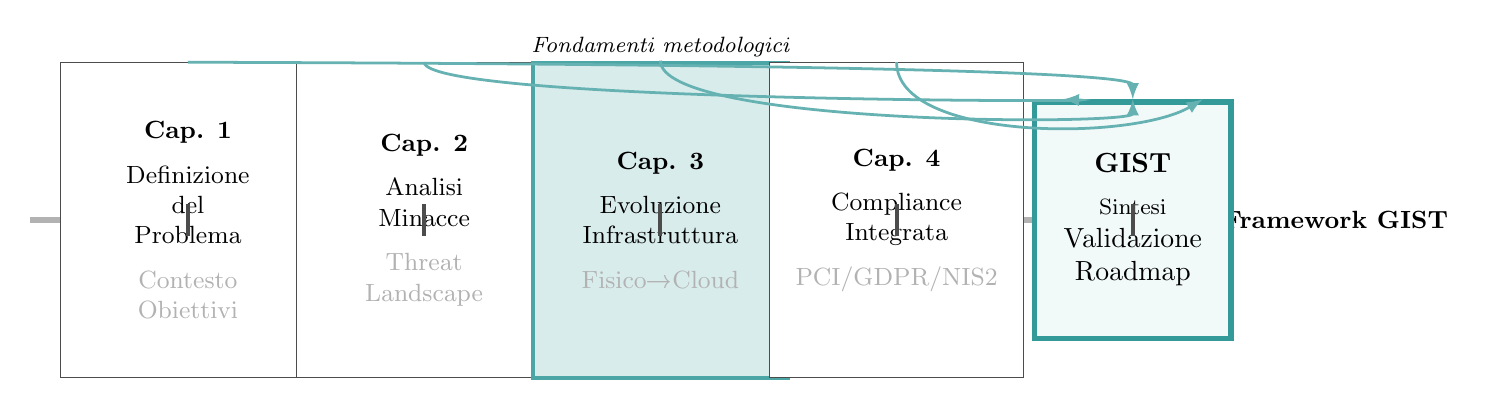
\begin{tikzpicture}[
    phase/.style={rectangle, draw=black!70, fill=white, text width=3cm, 
                  minimum height=4cm, align=center, font=\small},
    highlight/.style={fill=teal!15, draw=teal!70, line width=1.5pt},
    timeline/.style={->, >=stealth, line width=2pt, draw=gray!60},
    contribution/.style={->, >=latex, line width=1pt, draw=teal!60},
    label/.style={font=\footnotesize\itshape}
]

% Timeline principale
\draw[timeline] (0,0) -- (15,0) node[right] {\small \textbf{Framework GIST}};

% Fasi della ricerca
\node[phase] at (2,0) (intro) {
    \textbf{Cap. 1}\\[5pt]
    Definizione\\del\\Problema\\[5pt]
    \textcolor{gray!60}{Contesto\\Obiettivi}
};

\node[phase] at (5,0) (threat) {
    \textbf{Cap. 2}\\[5pt]
    Analisi\\Minacce\\[5pt]
    \textcolor{gray!60}{Threat\\Landscape}
};

\node[phase, highlight] at (8,0) (infra) {
    \textbf{Cap. 3}\\[5pt]
    Evoluzione\\Infrastruttura\\[5pt]
    \textcolor{gray!60}{Fisico→Cloud}
};

\node[phase] at (11,0) (compl) {
    \textbf{Cap. 4}\\[5pt]
    Compliance\\Integrata\\[5pt]
    \textcolor{gray!60}{PCI/GDPR/NIS2}
};

% Framework GIST
\node[rectangle, draw=teal!80, fill=teal!5, line width=2pt,
      minimum width=2.5cm, minimum height=3cm, align=center] at (14,0) (gist) {
    \textbf{GIST}\\[3pt]
    \footnotesize
    Sintesi\\Validazione\\Roadmap
};

% Contributi cumulativi
\draw[contribution] (intro.north) .. controls (2,2) and (14,2) .. 
    node[label, above, pos=0.5] {Fondamenti metodologici} (gist.north);
\draw[contribution] (threat.north) .. controls (5,1.5) and (14,1.5) .. (gist.120);
\draw[contribution] (infra.north) .. controls (8,1.2) and (14,1.2) .. (gist.90);
\draw[contribution] (compl.north) .. controls (11,1) and (14,1) .. (gist.60);

% Milestone indicators
\foreach \x in {2,5,8,11,14} {
    \draw[black!70, line width=1.5pt] (\x,-0.2) -- (\x,0.2);
}

\end{tikzpicture}
\caption{Progressione temporale della ricerca. Il capitolo evidenziato (Cap. 3) rappresenta il punto di svolta nell'integrazione delle componenti del Framework GIST.}
\label{fig:struttura_v2}
\end{figure}

% FIGURA 1.5 - VERSIONE 2: Matrix di impatto con heatmap
\begin{figure}[htbp]
\centering
\begin{tikzpicture}[
    cell/.style={rectangle, minimum width=3cm, minimum height=1.5cm, 
                 align=center, font=\small, draw=black!50},
    header/.style={cell, fill=gray!80, text=white, font=\small\bfseries},
    high/.style={cell, fill=red!60},
    medium/.style={cell, fill=yellow!50},
    low/.style={cell, fill=green!40}
]

% Headers
\node[header] at (0,0) {Dimensione};
\node[header] at (3,0) {Impatto Diretto};
\node[header] at (6,0) {Impatto Indiretto};
\node[header] at (9,0) {Metriche Chiave};

% Riga Accademica
\node[header] at (0,-1.5) {Accademica};
\node[high] at (3,-1.5) {Alto};
\node[medium] at (6,-1.5) {Medio};
\node[cell, fill=blue!20] at (9,-1.5) {
    4 modelli\\
    2 pattern
};

% Riga Pratica
\node[header] at (0,-3) {Pratica};
\node[high] at (3,-3) {Alto};
\node[high] at (6,-3) {Alto};
\node[cell, fill=blue!20] at (9,-3) {
    -35\% costi\\
    ROI 18 mesi
};

% Riga Sociale
\node[header] at (0,-4.5) {Sociale};
\node[medium] at (3,-4.5) {Medio};
\node[high] at (6,-4.5) {Alto};
\node[cell, fill=blue!20] at (9,-4.5) {
    45M utenti\\
    SLA 99.95\%
};

% Legenda
\node[rectangle, draw=black!50, align=left, below right=0.5cm and 0cm of current bounding box.south west] {
    \footnotesize
    \textbf{Legenda impatto:}
    \colorbox{red!60}{\phantom{xx}} Alto
    \colorbox{yellow!50}{\phantom{xx}} Medio  
    \colorbox{green!40}{\phantom{xx}} Basso
};

\end{tikzpicture}
\caption{Matrice di valutazione dell'impatto della ricerca. L'intensità del colore indica il livello di impatto previsto per ciascuna dimensione.}
\label{fig:impatto_v2}
\end{figure}

% ===================================================================
% VERSIONE 3: FIGURE CON STILE INFOGRAFICO MODERNO
% ===================================================================

% FIGURA 1.4 - VERSIONE 3: Diagramma a spirale evolutiva
\begin{figure}[htbp]
\centering
\begin{tikzpicture}[
    scale=0.8,
    transform shape,
    chapter/.style={circle, minimum size=2.5cm, align=center, 
                    font=\footnotesize\bfseries, draw, line width=1.5pt},
    arrow/.style={->, >=latex, line width=2pt, draw=blue!60}
]

% Definizione della spirale
\foreach \i/\angle/\radius/\color/\name in {
    1/90/2/blue!20/{Intro},
    2/180/2.8/blue!35/{Threat},
    3/270/3.6/blue!50/{Infra},
    4/360/4.4/blue!65/{Compl},
    5/450/5.2/blue!80/{GIST}
} {
    \node[chapter, fill=\color] (cap\i) at (\angle:\radius cm) {
        Cap. \i\\
        \name
    };
}

% Centro
\node[circle, fill=orange!80, text=white, minimum size=1.5cm, 
      font=\small\bfseries] at (0,0) {START};

% Connessioni a spirale
\draw[arrow] (0.75,0) arc (0:90:0.75) -- (cap1);
\draw[arrow] (cap1) arc (90:180:2) -- (cap2);
\draw[arrow] (cap2) arc (180:270:2.8) -- (cap3);
\draw[arrow] (cap3) arc (270:360:3.6) -- (cap4);
\draw[arrow] (cap4) arc (360:450:4.4) -- (cap5);

% Annotazioni
\node[align=center, font=\scriptsize] at (135:1.4) {Fondamenti};
\node[align=center, font=\scriptsize] at (225:2.4) {Analisi};
\node[align=center, font=\scriptsize] at (315:3.2) {Progettazione};
\node[align=center, font=\scriptsize] at (45:4) {Integrazione};
\node[align=center, font=\scriptsize] at (90:4.8) {Validazione};

% Framework components
\node[rectangle, rounded corners=5pt, draw=gray!70, fill=white,
      text width=3cm, align=center, font=\scriptsize,
      right=1cm of cap5] (components) {
    \textbf{Componenti GIST}\\[2pt]
    Physical (P)\\
    Architectural (A)\\
    Security (S)\\
    Compliance (C)
};

\draw[->, gray!50, dashed] (cap5) -- (components);

\end{tikzpicture}
\caption{Evoluzione a spirale della ricerca. Ogni capitolo amplia il raggio d'azione, culminando nel Framework GIST che integra tutti i contributi precedenti.}
\label{fig:struttura_v3}
\end{figure}

% FIGURA 1.5 - VERSIONE 3: Dashboard di impatto con KPI
\begin{figure}[htbp]
\centering
\begin{tikzpicture}[
    kpi/.style={rectangle, rounded corners=10pt, minimum width=4cm, 
                minimum height=2.5cm, align=center, font=\small, 
                draw=#1!70, fill=#1!10, line width=1.5pt},
    number/.style={font=\LARGE\bfseries, text=#1!80},
    label/.style={font=\footnotesize\itshape},
    icon/.style={font=\Large}
]

% Titolo
\node[font=\large\bfseries] at (6,0) {Dashboard Impatto Framework GIST};

% KPI Row 1
\node[kpi=blue] at (0,-2) {
    \icon{🎓}\\[2pt]
    \textbf{Pubblicazioni}\\
    \node[number=blue]{6}\\
    \label{Paper peer-reviewed}
};

\node[kpi=green] at (5,-2) {
    \icon{💰}\\[2pt]
    \textbf{Risparmio Costi}\\
    \node[number=green]{35\%}\\
    \label{Compliance integrata}
};

\node[kpi=orange] at (10,-2) {
    \icon{👥}\\[2pt]
    \textbf{Utenti Protetti}\\
    \node[number=orange]{45M}\\
    \label{Consumatori italiani}
};

% KPI Row 2
\node[kpi=purple] at (0,-5) {
    \icon{⏱️}\\[2pt]
    \textbf{ROI Medio}\\
    \node[number=purple]{18}\\
    \label{Mesi al break-even}
};

\node[kpi=red] at (5,-5) {
    \icon{🛡️}\\[2pt]
    \textbf{Riduzione Breach}\\
    \node[number=red]{40\%}\\
    \label{Incidenti evitati}
};

\node[kpi=teal] at (10,-5) {
    \icon{📈}\\[2pt]
    \textbf{Availability}\\
    \node[number=teal]{99.95\%}\\
    \label{SLA garantito}
};

% Footer con trend
\node[rectangle, draw=gray!50, fill=gray!5, text width=12cm,
      align=center, below=1cm of current bounding box.south] {
    \footnotesize
    \textbf{Trend 2024-2025:} ↑ Adozione +67\% | ↓ Costi IT -23\% | ↑ Minacce +312\%
};

\end{tikzpicture}
\caption{Dashboard degli indicatori chiave di performance (KPI) del Framework GIST. I valori rappresentano impatti misurabili validati attraverso analisi empirica.}
\label{fig:impatto_v3}
\end{figure}